\chapter{Apparatus}
\label{Chap_Apparatus}

% epigraph (done 2021-8-24 09:23:49)
\setlength{\unitlength}{1pt}
\setlength{\epigraphwidth}{10.5cm}
\epigraph{工欲善其事,必先利其器。\\ A craftsman must sharpen his tools to do his job. \cite{Confucius1993Ta}}{--- Confucius\\ \textit{The Analects (5th century BC)}}

% introduction (NOT done renew this one after finish the rest)
This chapter describes the Na-Rb machine and the upgrades we have done for our droplet experiment. As most of the setup has been described by the previous thesis \cite{WangFudong2016Soau,LiXiaoke2015Chsd}, we only shortly make a summary in Sec. \ref{sec:machine} for the completeness of this chapter. In Sec. \ref{sec:image}, we turn to the image system upgrades for measuring the droplet sample with several $\mu$m sizes. We design a 15$\times$ image system with a resolution of 2$\mu$m level. Besides, we upgraded the mechanical part onto an electro-translation stage, which can follow the ToF of the free-falling sample without worsening the image resolution. We detailedly describe the high-magnetic field in-situ image scheme for subtracting the sample's density profile reliable. Finally, we discuss several improvements such as fast-coil for fast controlling magnetic field (Sec. \ref{sec:fastcoil}), magnetic field gradient compensation (Sec. \ref{subsec:gradientcompen}) and coil antennas for increasing the Rabi frequency of Rb (Na) micro-wave transition (Sec. \ref{subsec:FWLA}).

\section{Overview: Na-Rb machine I}
\label{sec:machine}

% goal of this Na-Rb machine (done 2021-8-24 10:28:43)
A cold atom machine that can produce repeatable samples with stable atomic conditions is essential to carry out the following experiments. So, even though the Na-Rb machine in our laboratory has been running for longer than eight years, many aspects still need to improve to make the sample condition more stable. \cite{LiLintao2021} describes many efforts we made: optimization of the micro-wave evaporation procedure for Rb sympathies cooling of Na; a new ultra-stable magnetic field servo system for achieving hundred-Gauss with only two mG level fluctuation. Besides stability, more atom is another goal for many experiments because there are always various types of loss in producing the atomic (or molecular) samples. The final sample with more numbers can make detection easier. In the droplet experiment, if we produce a sample with ten times more numbers (i.e. $10^6$ for each species), we can study more properties of the bulk sample, such as flat-top density profile \cite{petrov2015}, the surface excitation modes \cite{petrov2015} and achieving a longer lifetime.

缺少一个整体的图片,加入整体的设计图片

\subsection{Production of Na-Rb Bose-Einstein condensate mixtures}

% dispenser (done 2021-8-25 10:24:28)
\begin{figure}[htb]
\begin{center}
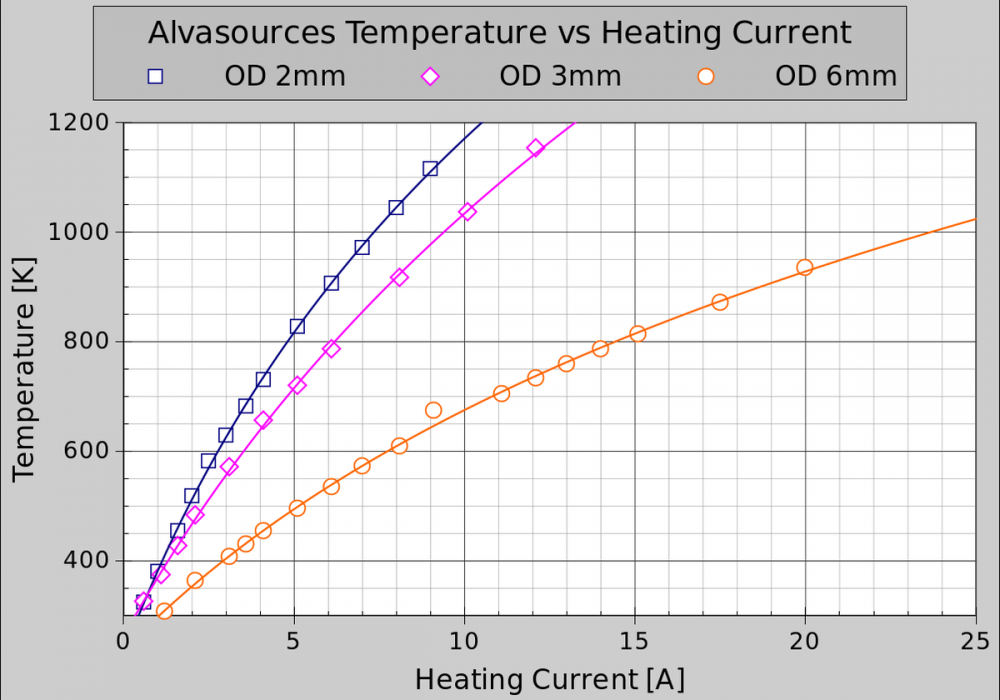
\includegraphics[width = 0.7\linewidth]{figures/Apparatus_dispen.png}
\end{center}
\caption[Temperature-current relationship of dispenser (Image from \href{https://alfavakuo.eu/products/mvs/}{alfavakuo})]{Temperature-current relationship of dispenser (Image from \href{https://alfavakuo.eu/products/mvs/}{alfavakuo}). The dispenser of Na and Rb are both with diameter of 3 mm.}
\label{Apparatus_dispen}
\end{figure}

% Dispenser, LIAD method for loading (done 2021-8-25 11:00:14)
Our experiment starts from Na and Rb dispensers. We fire the Rb dispenser every day with a relatively low current of 1.9 A (temperature of less than 500 K). Na dispenser fires only once a month, however, with a relatively high current (3.5 A) and temperature (600 K). The temperature and current conversion chart is shown in Fig, \ref{Apparatus_dispen}. The reason for not firing the Na dispenser at a low current is that the temperature for turning on the Na dispenser (Na starts to spray out) is still too high and breaks the vacuum. Since we use a single chamber design, we have to make the trade-off between the loading rate of MOT and the vacuum condition. Thanks to the light-induced atomic desorption (LIAD) method, the glass wall can absorb the atoms when UV light is off. Then, by turning UV on, we can increase the atoms flux (for both Rb and Na) for MOT loading at the beginning of each shot. Of course, this will degrade the vacuum condition in the chamber, however, after MOT loading, we turn off the UV, and the atom can be absorbed again by the chamber and then the vacuum recovers. The typical lifetime of Rb in the quadruple trap (QT) is 30 s level, and Optical-trap (OT) lifetime is about 20 s. 

% CMOT, molasses (done 2021-8-26 14:28:05)
After atoms gradually accumulating within 30 seconds, Na and Rb MOT finally achieves saturation. To avoid collision between Rb and Na that induces an inelastic process, we use a resonance light to push the Rb MOT aside to avoid overlapping Na and Rb. That dual MOT typically can capture $10^{9}$ Rb and $1.5 \times 10^{6}$ Na. To increase its density, we apply a compress-MOT (CMOT) process, which increases the restoring force by far detuning the MOT laser\footnote{in our experiment, we do not increase the magnetic gradient.}. To further increase the phase space density (PSD) of the sample, a molasses process is implemented to cool the sample further. Finally, we load the sample into QT with both species in $\ket{F=1,m_F=-1}$ state.

% In QT and QT evaporation and hybrid trap (done 2021-8-26 14:53:38)
A pair of the anti-Helmholtz coil generates the Quadrupole trap (QT). At the beginning of the time sequence, the magnetic gradient is ramped up to 160 G/cm, served as a conservation trap for capture all atoms from the precooling stage. Then, we do the evaporation cooling for Rb which using a MW to pump atoms from $\ket{F=1,m_F=-1}$ to $\ket{F=2,m_F=0}$. Due to the anti-trapping of $\ket{F=2,m_F=0}$ state, we can remove the high-temperature atoms away from the trap to decrease the overall sample temperature. Na atoms are sympathetically cooled by Rb. Due to Majorana loss bringing anti-evaporation effect, we add a single beam optical trap to shift the minimum position of the whole potential away from the QT centre. This works at the first evaporation stage and helps us obtain a sample with 20 $\mu$ K temperature. After that, we adiabatically lower down the QT to 26 G/cm for avoiding severe Majorana loss further. After the MW sweeping to 6833 MHz, we finally achieve a mixture sample with temperature around several $\mu$K. This allows us to load them to an Optical dipole trap to do further cooling and experiment. More details about this hybrid trap can be found in this note of our lab \cite{xiong2013production}.

% In OT and OT evaporation (done 2021-8-26 15:09:24)
Optical trap evaporation is achieved by forcibly reducing the light intensity. In the later stage, the atomic density becomes lower due to the weakening of confinement, which reduces the collision rate, so a slower evaporation rate is required. As a result, the optical trap evaporation is relatively inefficient. Using 1070 crossed OT in our experiment, we typically spend 3 s to obtain a two-species BEC. For a one-dimensional optical trap, the evaporation time requires even longer and may take 5-10s. Therefore, we generally obtain BEC in the 1070 XOT first and then transfer it to other types of optical traps for experiments. Of course, the transfer process will inevitably bring excitation, so it is crucial to deceive an adiabatic process or wait a long enough time for reaching the ground state.

% state preparation (done 2021-8-26 20:11:43)
Since we need the Feshbach resonance between Na and Rb both in  $\ket{F=1,m_F=1}$ state, we need transfer atoms from $\ket{F=1,m_F=-1}$ to the target state. The easiest and most robust way is the adiabatic-rapid passage (ARP). By applying an RF(or MW) field to couple the initial and target state, we can detune its detuning from the blue (red) side to the red (blue) side. Following the dressed state, atoms start from $\ket{F=1,m_F=-1}$ however end with $\ket{F=1,m_F=1}$. This procedure needs enough adiabaticity, which is time-consuming; however, it is robust from the system's power fluctuation and time precision. We carry out the transition under a low magnetic field, which enables us couple the $\ket{F=1,m_F=-1}$ state to $\ket{F=1,m_F=0}$ and then to $\ket{F=1,m_F=1}$. For latter experiments that need $\ket{F=1,m_F=0}$, we can apply a relatively high magnetic field to decouple these two transitions. More details can be found in the previous thesis \cite{WangFudong2016Soau,LiXiaoke2015Chsd,LiLintao2021}.

% 1070 and 946 ODT (done 2021-8-26 15:24:14)
\begin{figure}[htb]
\begin{center}
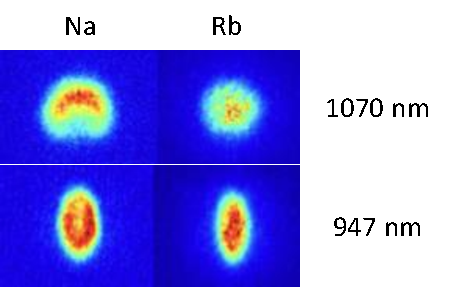
\includegraphics[width = 0.6\linewidth]{figures/OT_1070-946.pdf}
\end{center}
\caption[Na and Rb samples in 946 and 1070 nm ODT (image from \cite{LiLintao2021})]{考虑换成947也是圆形trap的照片 Na and Rb samples in 946 and 1070 nm ODT (image from \cite{LiLintao2021}). Due to gravitational sag difference, Na in 1070 ODT is buoyant above Rb. In 946 nm ODT, Rb stays at the centre of Na, showing the sag difference's excellent compensation.}
\label{OT_1070-946}
\end{figure}

% BEC mixture (done 2021-8-26 16:49:43)
In our experiment, Na has a relatively large scattering strength $g_{Na}$, so at the beginning of OT evaporation, it is Na sympathetically cooling Rb. However, typically Na becomes BEC before Rb does because of a higher transition temperature, which is mainly due to the higher trap frequency of Na in the 1070 nm ODT. After that, the evaporation is mainly for the Rb sample, and we can achieve a two-species BEC with an almost balanced number at the final. This number ratio actually can be tuned by changing the evaporation ending in QT. For the double BEC sample in ODT, Na is immiscible with Rb in the case of a low magnetic field. Thus, Na shows a crescent shape which is because of the gravitational sag difference of two samples (shown in Fig. \ref{OT_1070-946}). In order to obtain a relatively pure BEC sample, we lower down the optical trap to a relatively shallow level, such as about 80 Hz for Na in 1070 ODT. We check the purity of the BEC sample by observing the BEC sample without any thermal part for whatever ToF. Then, we say that the sample is pure enough. However, to characterize the temperature of this sample, correspondingly the BEC fraction, is typically hard, which is beyond the range of this thesis.

% number ratio control (done 2021-8-26 17:54:39)
In many experiments, we need to control the number ratio of Na and Rb. The typical method is to adjust the optical trap's relative position to the QT's zero-point. By modifying this distance, we can determine the atomic number of Rb after the QT evaporation. Rb will be less evaporated and more Rb atoms remain for a longer distance, vice versa. Because the Na number is much less than Rb, with sympathetically cooled, the Na number mainly unchanges. However, the temperature will be the same as Rb. Subsequently, the evaporation of loading into OT is dominated by Na, as mentioned before. Therefore, the number ratio of Na and Rb can be manipulated by changing the number of the remaining Rb after QT evaporation.

% 946 trap (done 2021-8-27 10:40:15)
As described in \cite{LiLintao2021}, we build an optical trap with magic wavelength, which offers the same trap frequency for both Na and Rb. As shown in Fig. \ref{OT_1070-946}, Rb stays at the centre of Na. We can benefit a lot from this wavelength, such as increasing the overlap between Na and Rb and consequently increasing the Feshbach molecule's conversion rate or enhancing the signal of the polaron experiment. Our droplet experiment uses this sag-difference-free trap to achieve better overlap and form droplets with lower density and longer lifetime, which will be discussed in Chap. \ref{Chap_droplet}.

\subsection{Production of Na-Rb Feshbach molecules}
% motivation (done 2021-8-26 18:49:35)
In our laboratory, the original intention of producing Feshbach molecules is to make the ground state molecule of NaRb further. After successfully making the ground state molecule \cite{}, the mission of this machine becomes the study of heteronuclear mixture BEC. The core ingredient of research on this set-up consequently involves adjusting inter-particle interaction through the Feshbach resonance. Many interesting physics problems can be studied, such as Effimov state, polaron, spinor. Then the essential parameter is the FR parameter, i.e. how the scattering length of the inter-species changes with the magnetic field. The detailed calibration and calculation will be demonstrated in Chap. \ref{Chap_Feshbach}. We note that the scattering properties near resonance will be most affected by the shallowest bound state, so the precision measurement of the bound state will give accurate scattering properties in turn. Therefore, we need to synthesize FR molecules and study their properties.

% method (done 2021-8-27 10:40:51)
Our experiment starts from an optically trapped ultracold mixture of $^{23}$Na and $^{87}$Rb atoms, both in their lowest hyperfine state $\ket{F = 1, m_F = 1}$~\cite{wang2013observation,wang2015formation,jia2020}. Magnetoassociation starts from an initial magnetic field of 350 G, just above the FR at $B_0 = 347.64$ G. The magnetic field is ramped down across the resonance to form FMs, and then to 335.6 G. At this field, the FMs have a nearly zero magnetic dipole moment; this allows us to remove the residual atoms with a short and strong magnetic field gradient without losing molecules. Afterwards, the magnetic field is ramped up to a range of target values below $B_0$ for further experiments. Following this procedure, we can routinely obtain a pure sample of \NaRb~FMs with a typical temperature of 300 nK and a trap lifetime of more than 30 ms. This short lifetime is due to near-resonance photon scattering by the 947 nm optical trap light~\cite{Guo2017,jia2020}, which is provided by a home-built diode laser system. In another experiment on \NaRb, in which a single-frequency 1064 nm laser is used as the optical trap light, FM lifetimes greater than 100 ms have been observed~\cite{Wang2019,guo2021leehuangyang}. Nevertheless, the current lifetime is more than enough for the present work, as we need only 10 ms for magnetic field stabilization and less than 1 ms for dissociation.

\section{Image system upgrades}
\label{sec:image}

% motivation: why upgrade image system (done 2021-8-27 11:04:57)
The previous image system is composed of an f=100mm (\#49360-INK) and f=300 mm (\#49368-INK) pair from Edmund optics, which can support a resolution of about 3 $\mu$m (N.A.=0.13) as shown in Fig. \ref{old_image}. This imaging system is built with discrete elements, which cannot be moved as a whole. Thus, it is only proper for imaging for a small region; otherwise, both spherical aberration and coma shows up if moving only the camera or the lens set. We need to do the ToF for samples for the droplet experiment, and the displacement reaches about 2 mm. If we change the camera position, the resolution for imaging sample with large displacement, i.e. at the edge of field-of-view, will be degraded. So, we improved our resolution by two means: First, we increase the imaging system's resolution by using a long working distance objective; secondly, we build a whole block by mounting all optical elements and cameras onto an electric translation stage. In the rest of this section, we discuss the absorption image method for a dense atomic cloud, introduce a high-magnetic-field image scheme, and discuss the number calibration method.

% old imaging system: left Zemax, right picture
%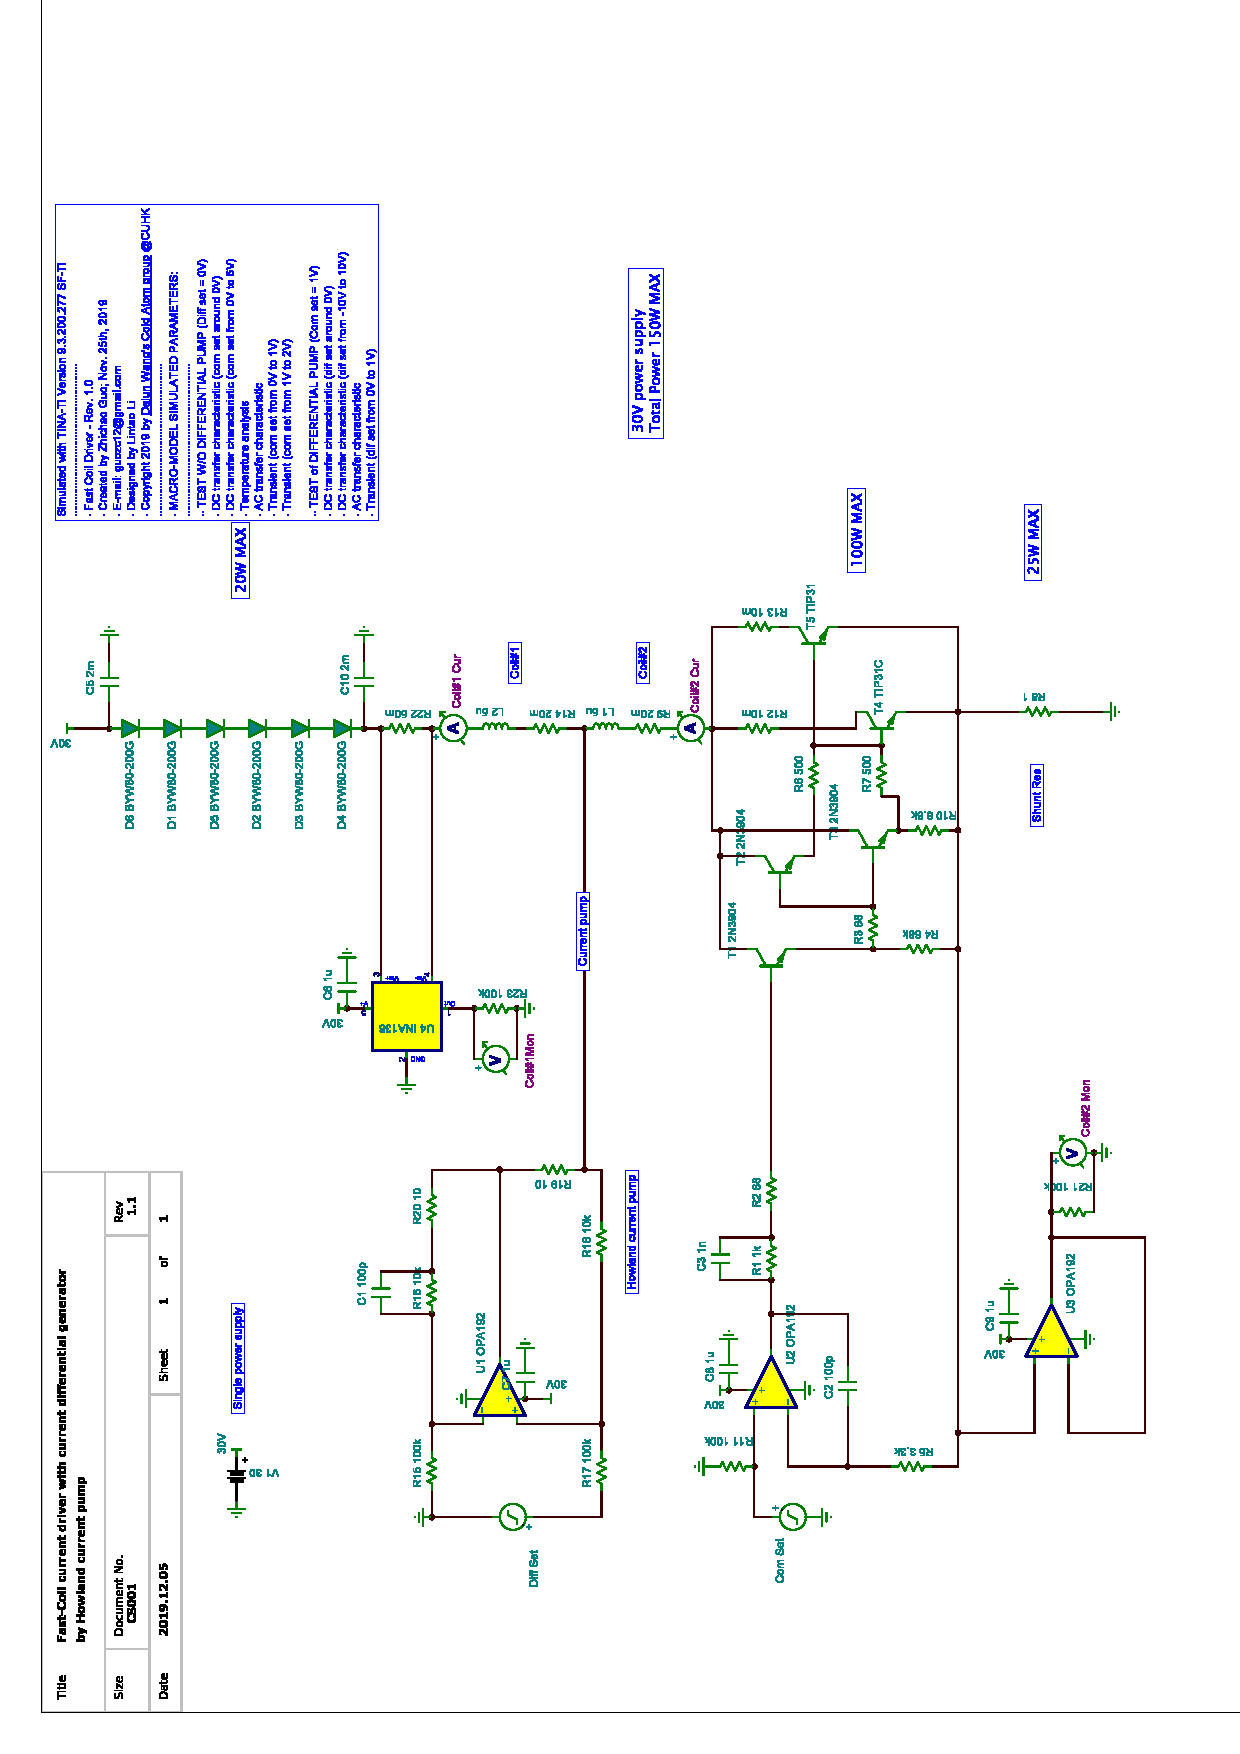
\includepdf[addtotoc={1,section,1,title in toc,cc},pages=1-4,offset=0cm 0.5cm]{FastCoilDriver-SimuTinati.pdf}
\begin{figure}[htbp]
\begin{center}
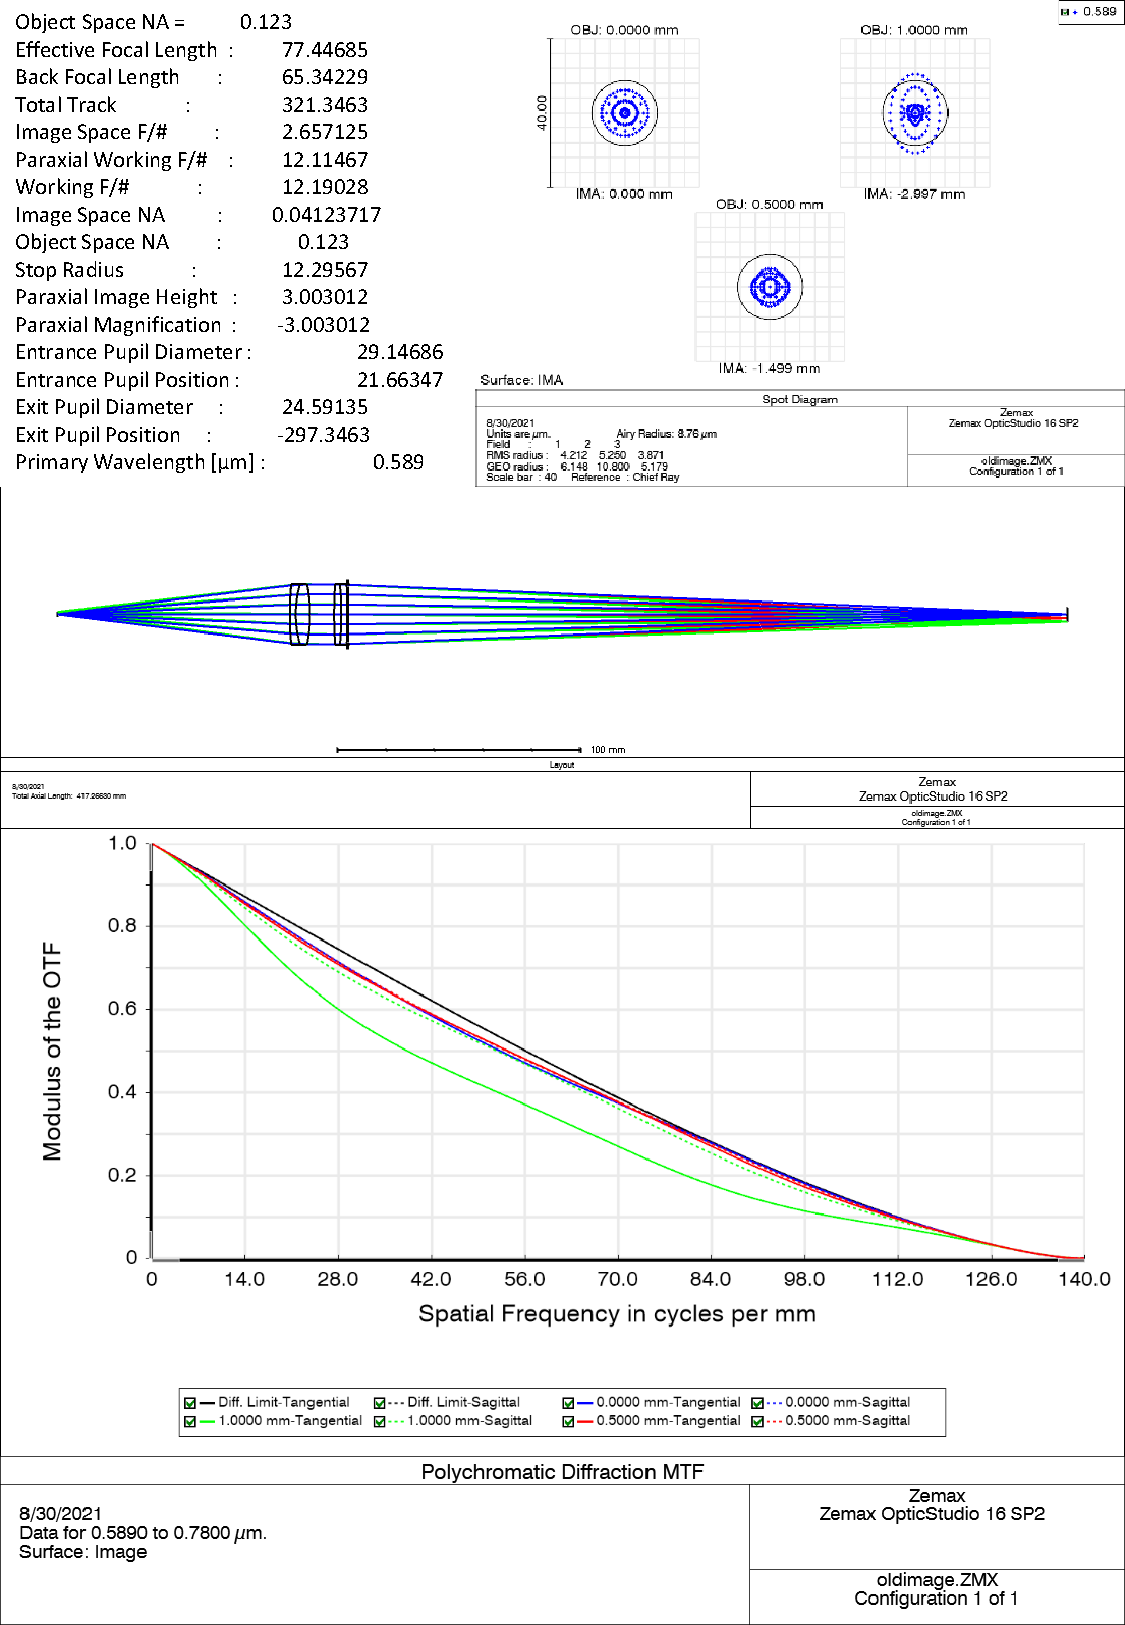
\includegraphics[width = \linewidth]{figures/old image.pdf}
\end{center}
\caption[3x image system simulation by Zemax]{3x image system simulation by Zemax}
\label{old_image}
\end{figure}

\subsection{High resolution image system}
% optical design (done 2021-8-27 14:44:36)
The characteristic length for a droplet is typical of several $\mu$m, as shown in Sec. \ref{Chap_droplet}. In order to resolve this tiny sample, we need a better imaging system with resolution reaching $\mu$m level. The old imaging system with an f=100mm objective is not enough since its N.A. is 0.13 with an airy radius of about 4 $\mu$m. So, we use an objective with a shorter focal length to increase N.A. The most convenient way is using a microscope with a long working distance. So, we choose a 10X Mitutoyo plan-apo infinity-corrected Long-WD objective with an effective focal length of 20 mm. Its working distance reaches 34 mm, enough for our application without blocking any optical path, such as MOT or optical trap. We can use the same eyepiece (Edmund \#49368) with f=300 mm and directly image the atom onto the camera thanks to the infinity-correction property. 

% Zemax simulation
To further understand the behaviour of the new image system, and to check whether the cell glass destroy the image quality, we imply a Zemax simulation for this new image system. As shown in Fig. \ref{zemax_image}, ......


% Zemax simulation for High-field image scheme
\begin{figure}[htb]
\begin{center}
\includegraphics[width = 0.8\linewidth]{figures/zemax_image.pdf}
\end{center}
\caption[15x new image system design]{15x new image system design}
\label{zemax_image}
\end{figure}

% mechanical design (done 2021-8-27 15:09:52)
As shown in Fig. \ref{image_system}, We use the cage system from Thorlabs to build the main body of the imaging system. A $45^\circ$ mirror reflects the probe beam in the vertical direction. This avoids the diffraction light from optical dipole trap scattering to CCD and affects the image quality. The dichromatic mirror can be tuned to ensure the Na image is at the centre of Na CCD. Moreover, we add a ring adjuster for Rb CCD to fine-tune its position. This is mainly for focusing on both Na and Rb. Because there always be a chromatic shift for two different wavelengths (589 nm for Na and 780 nm for Rb). So, when focusing on the system, we first focus the Na by move the set-up as a whole, i.e. move the objective on focus to the atom. Then, we tune the ring adjuster to focus Rb onto the camera. One mistake is that we choose an adjuster too fine (4 mm for ten turns), so the adjustment procedure typical take a long time. As mentioned before, the whole system is mounted onto an electric translation stage controlled by an Arduino. Code and control can be found in Lintao's thesis \cite{LiLintao2021}.

% High-field image scheme (done 2021-8-27 15:12:52)
\begin{figure}[htb]
\begin{center}
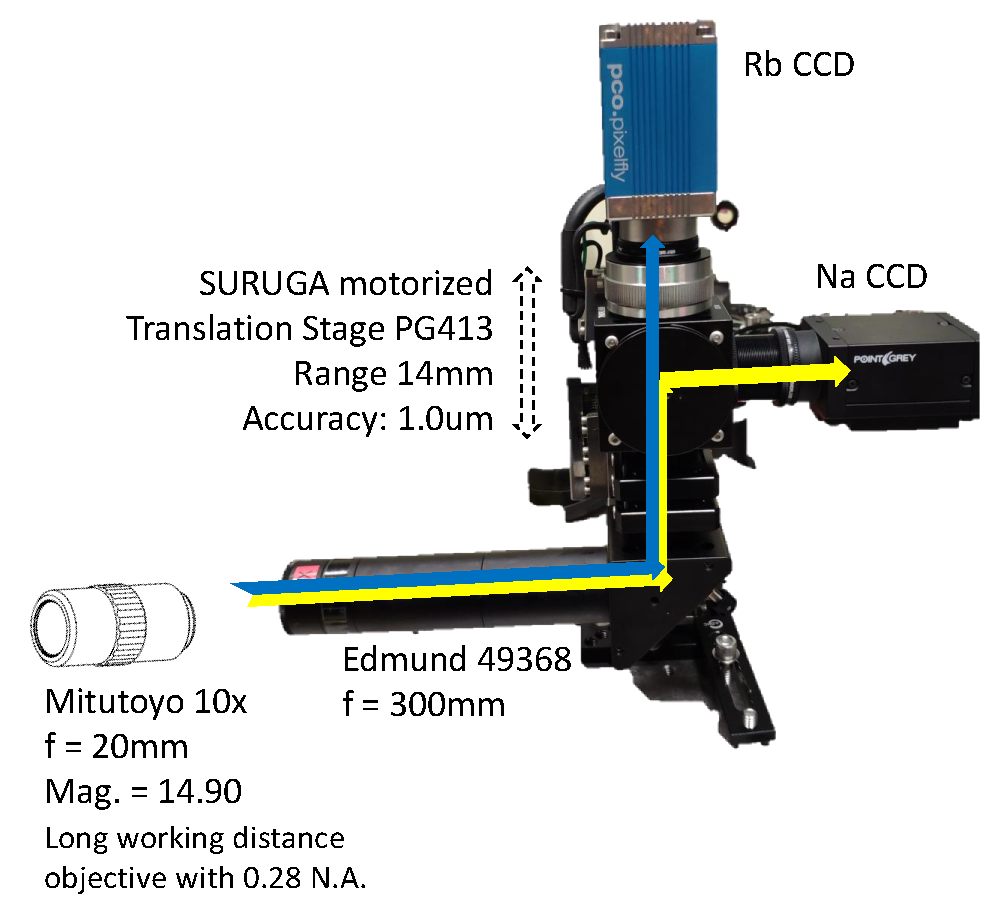
\includegraphics[width = 0.8\linewidth]{figures/image_system.pdf}
\end{center}
\caption[New compact imaging system]{New compact imaging system. The whole set-up is mounted on a electric translation stage from SURUGA. The objective can be switched between a Mitutoyo 10x microscope and a typical f=100 mm achromatic lens. Then follows a f=300 mm eyepiece for focusing. A dichromatic mirror splits Rb and Na probe into two CCDs.}
\label{image_system}
\end{figure}

% cell wall effect (done 2021-8-27 15:35:56)
Even though we use a powerful objective with an Airy radius of 1 $\mu$m, there exists a critical issue that the cell wall is 3 mm thick. So, we need to check the imaging system's performance with this 3 mm window before the objective. We do not do any correction for this glass wall because our primary goal is to increase the magnification. Even the resolution only increase twice will be enough for observing droplet signals. The 3mm window will decrease the resolution \footnote{A tutorial for standard object correction ring can be found \href{ http://www.mvi-inc.com/wp-content/uploads/Use-of-the-Correction-Ring-on-the-Objective.pdf}{here}. Moreover, the effects of thick glass on an imaging system can be found on \href{https://www.thorlabs.com/newgrouppage9.cfm?objectgroup_id=9895&pn=TL2X-SAP}{Thorlabs} under the tag of correction collar}. Since when the focused beam goes through the glass wall, light with a different angle will bend by different amplitude and finally, they cannot converge to a single point as without the glass. This effect is severe when the N.A. goes higher. So, first, we try to simulate the system with Zemax. As shown in Fig. \ref{}, two with and without the 3 mm window. The resolution can be found to increase to 1.5 um(check) when adding the 3mm glass. This is also enough for our droplet experiment. So we carry out this setup.

% resolution test
\begin{figure}[htb]
\begin{center}
\includegraphics[width = 0.8\linewidth]{figures/image_reso.pdf}
\end{center}
\caption[Test of image resolution of 15x image system]{image resolution}
\label{image_reso}
\end{figure}

% test resolution (done 2021-8-27 15:49:18)
Before putting it online, we first test its resolution offline with a USAF1951 target and 2 $\mu$m pinhole. Here, we show the measured Airy disk in Fig. \ref{image_reso}. By simply fitting the pattern with the Airy function, we get the resolution for Na(Rb) is 1.7(2.3) $\mu$m. So we now have a high resolution and commercial and cheap image system. 

% Translation stage (done 2021-8-27 16:44:06)
Because we will do ToF measurement for several tens of ms, i.e. about 2 mm away from the centre of view-of-field, spherical aberration and coma can worsen the image quality. This can be shown by Zemax by a tilted angle of input light (Fig. \ref{image_reso}). We use a high magnification imaging system with a short focal length of 20 mm. This makes its field-of-view very small. So, we need to move the whole imaging system along with the atomic sample. So, we build the imaging system very compact and mount it onto a translation stage controlled by a computer. The translation stage is mounted vertically with a step resolution of 1 $\mu$m. We use an Arduino board to control the driver. Finally, we can change the position of our image system at will shot by shot. To avoid the movement changing affecting the EM field around the cell, we make each movement at the interval of two shots.

\subsection{High magnetic field absorption image}

% SNR vs OD
\begin{figure}[htb]
\begin{center}
\includegraphics[width = 0.8\linewidth]{figures/SNR_OD.pdf}
\end{center}
\caption[SNR OD]{SNR OD}
\label{SNR_OD}
\end{figure}

% goal (done 2021-8-27 16:47:15)
To probe the droplet without distortion, we need the imaging scheme reliable, which means the method can recover the density profile of the sample as accurate as possible. Since a typical droplet sample has OD above 50 for Rb and 10 for Na, a typical absorption image method cannot be used directly, which is because the absorption image's SNR is limited when the sample OD is too high. As plotted in Fig. \ref{SNR_OD}, weak probe intensity (less than one saturation intensity) can only support OD smaller than 3. Increasing the probe intensity to achieve the saturation absorption image can increase the threshold of OD to probe. However, higher intensity could cause several other problems: first, calibration could be hard to do or cause a significant error because the nonlinear response of the absorption. second, for a high density sample the re-scattering problem could introduce the effect beyond the aforementioned theory. So, we conceive a partial pumping method and a high-magnetic field absorption imaging scheme for the high-OD samples.

% High-field image scheme (done 2021-8-27 16:52:34)
\begin{figure}[htbp]
\begin{center}
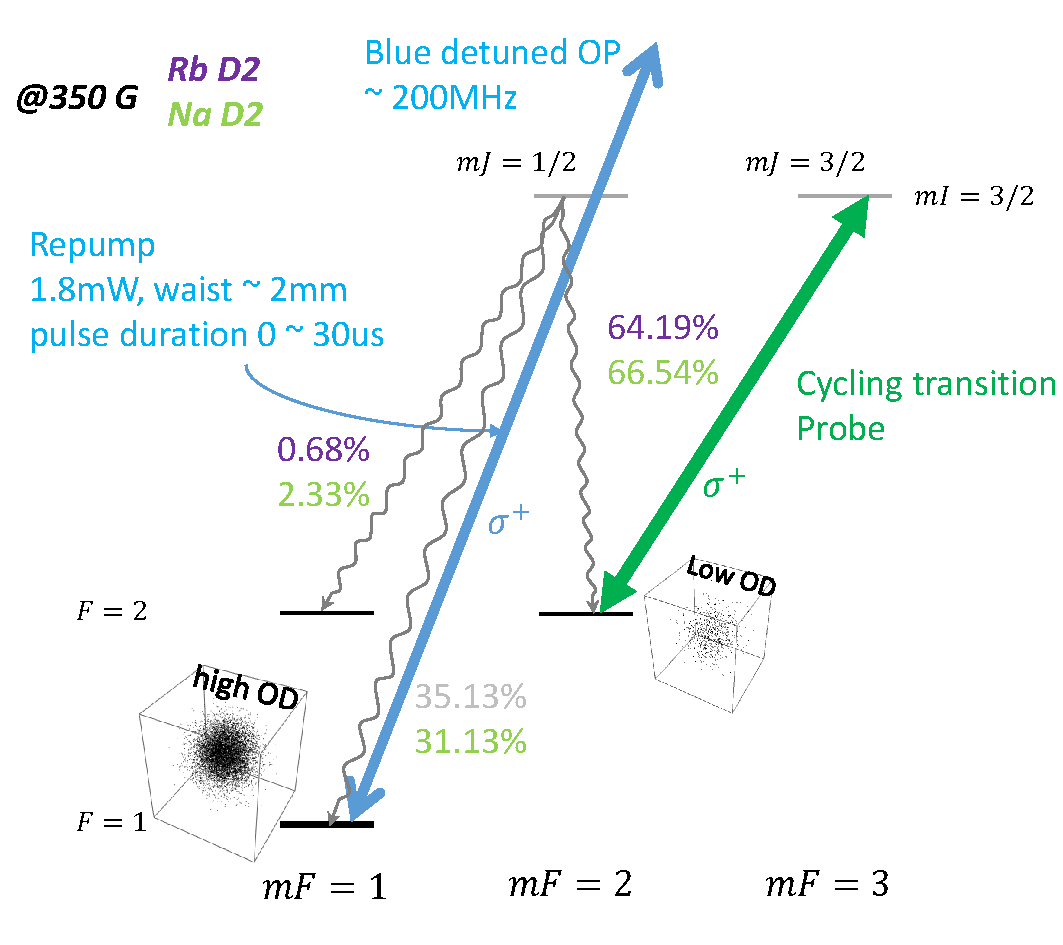
\includegraphics[width = 0.8\linewidth]{figures/High-field image scheme.pdf}
\end{center}
\caption[image scheme for Na(Rb) $\ket{F=1,m_F=1}$ state under 350 G magnetic field]{image scheme for Na(Rb) $\ket{F=1,m_F=1}$ state under 350 G magnetic field. The ground states are labelled with F and $m_F$; the excited states are labelled with $m_J$ and $m_I$. The imaging procedure is divided into two steps: first, pumping atoms from $\ket{F=1,m_F=1}$ to $\ket{m_J=1/2,m_I=3/2}$. After atoms accumulating to $\ket{F=2,m_F=2}$ state, we drive the cycling transition for absorption image. By blue detuning about 200 MHz of the pumping light, we can control the pumping ratio to control the OD for the image transition.}
\label{High-field image sheme}
\end{figure}

% image scheme (done 2021-8-27 17:47:45)
Thus, we first decrease the sample's density; however, we keep its profile unchanged. Then, we apply the typical absorption image. This is what we called the partial pumping method for absorption image. A typical way to pump a small portion of the sample to the image transition is by MW or light. As shown in Fig. \ref{image_system}, our sample is at $\ket{F=1,mF=1}$ state, which is non reacting with the absorption light. Then, we use a pumping laser to pump atoms to exited state $\ket{m_J=1/2,m_I=3/2}$; then, with spontaneous radiation, atoms accumulate onto $\ket{F=2,m_F=2}$ state. Finally, we use the cycling transition from this state to $\ket{m_J=3/2,m_I=3/2}$ state to do the absorption image. Here the pumping can also be done by the MW pulse. However, our original MW had a Rabi freq less than 10 kHz, which could consume 100 $\mu$s or even longer apply a $\pi$ pulse. This would make the sample's shape changed a lot when we probe it by the image light. We will get back to this point when we discuss our upgrades of the Full-wave loop-antenna in Sec. \ref{subsec:FWLA}. 

% partial_pumping (done 2021-8-27 17:50:32)
\begin{figure}[htb]
\begin{center}
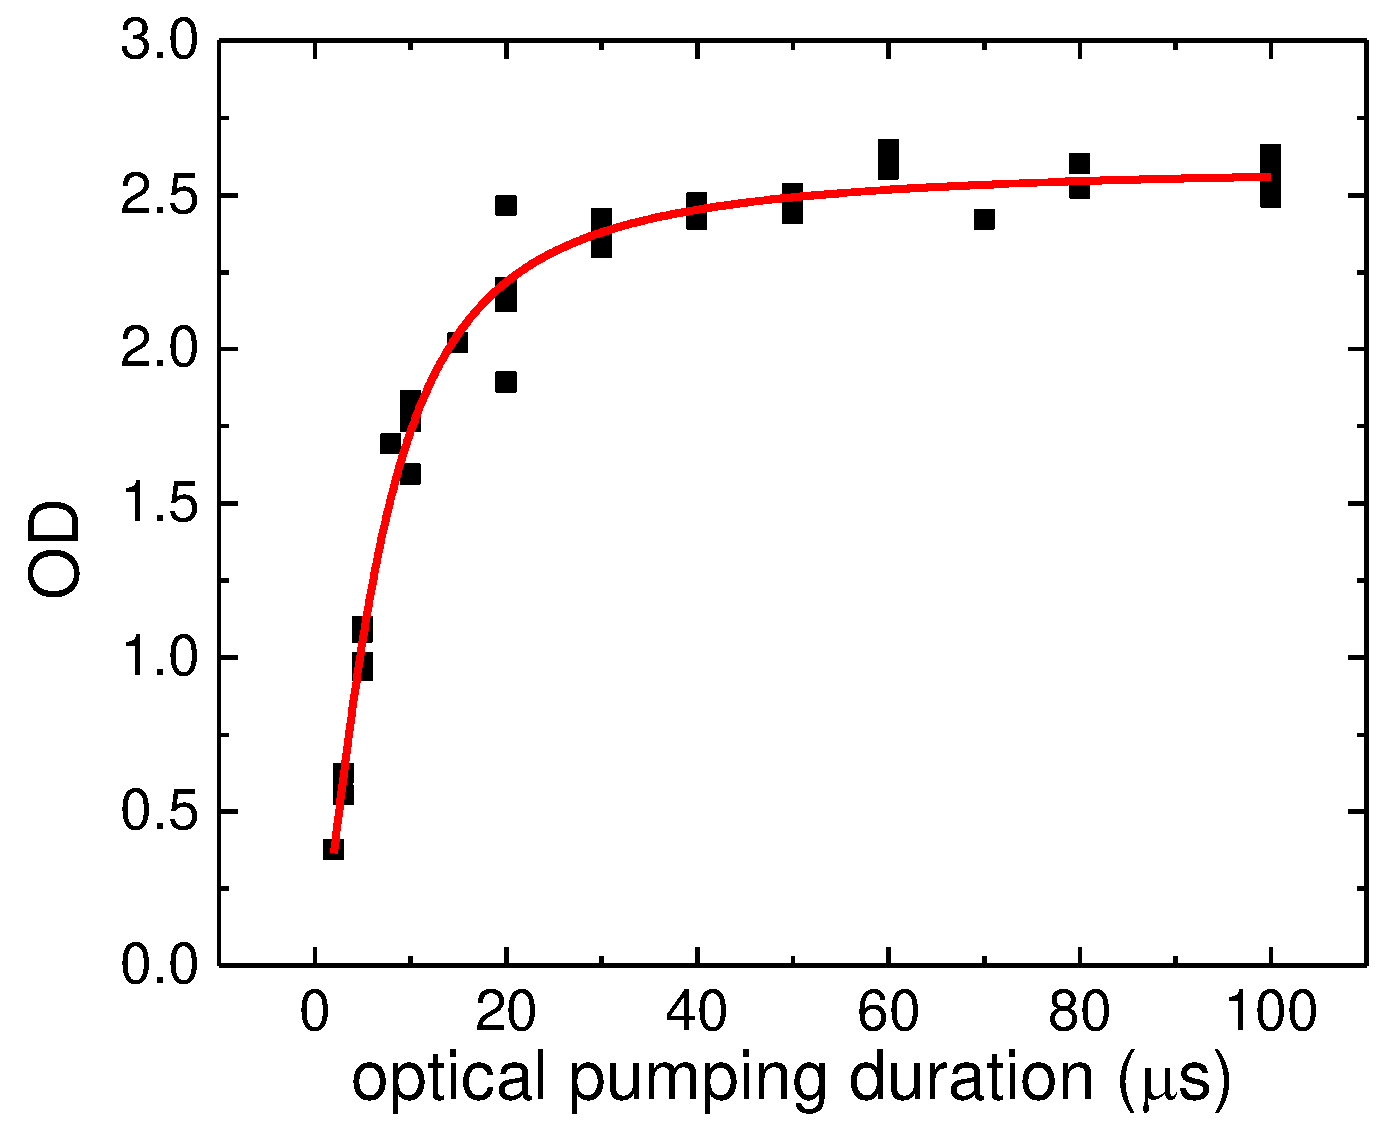
\includegraphics[width = 0.8\linewidth]{figures/partial_pumping.pdf}
\end{center}
\caption[Partial pumping portion as function of pump duration]{Partial pumping portion as a function of pump duration. Here shows the partial pumping for Na with 200 MHz blue detuning of the pumping light.}
\label{partial_pumping}
\end{figure}

% partial pumping (done 2021-8-27 18:02:39)
So, we choose the pumping laser instead of tuned to on resonance, and we make it large detuned away from the transition and make its intensity high. This method ensures the whole sample feel around the same intensity because large detuning and intensity make the atoms only absorb a tiny portion of the light. Even for a very dense sample, the unevenness of the saturation effect can be avoided. As plotted in Fig. \ref{image_scheme}, Na partial pumping a small portion of the sample to $\ket{F=2,m_F=2}$ state, which then can be detected directly. The pumping ratio can be controlled by the duration of the pumping laser. As shown in Fig. \ref{}, the OD of pumped Na atoms as a function of the pumping duration is plotted. We can see that we have an almost linear pumping speed for the first several tens of us, and after 50 $\mu$s we have a saturation effect. This saturation effect is used to calibrate latterly. For our experiment, to decrease the OD to less than 3, we typical using a detuning 200-300(check)MHz and pumping only several $\mu$s to achieve a portion less than 10 per cent. Then a typical low-intensity absorption image can afford it.

\subsection{Atomic number calibration}

% goal
As we want to not only measure the size of the sample but also the number of sample to get the critical number of the droplet. So, a reliable recovery of its number is important. This need a carefully calibration of the sample's number. As fomulated (add) the main parameters is the alpha which describe the ratio between effective saturation intensity and the calculated saturated intensity I0, or the ratio betweent he effective cross section and the sigma0. (need restate) 
% not finished

% Image_beta_calibration
\begin{figure}[htb]
\begin{center}
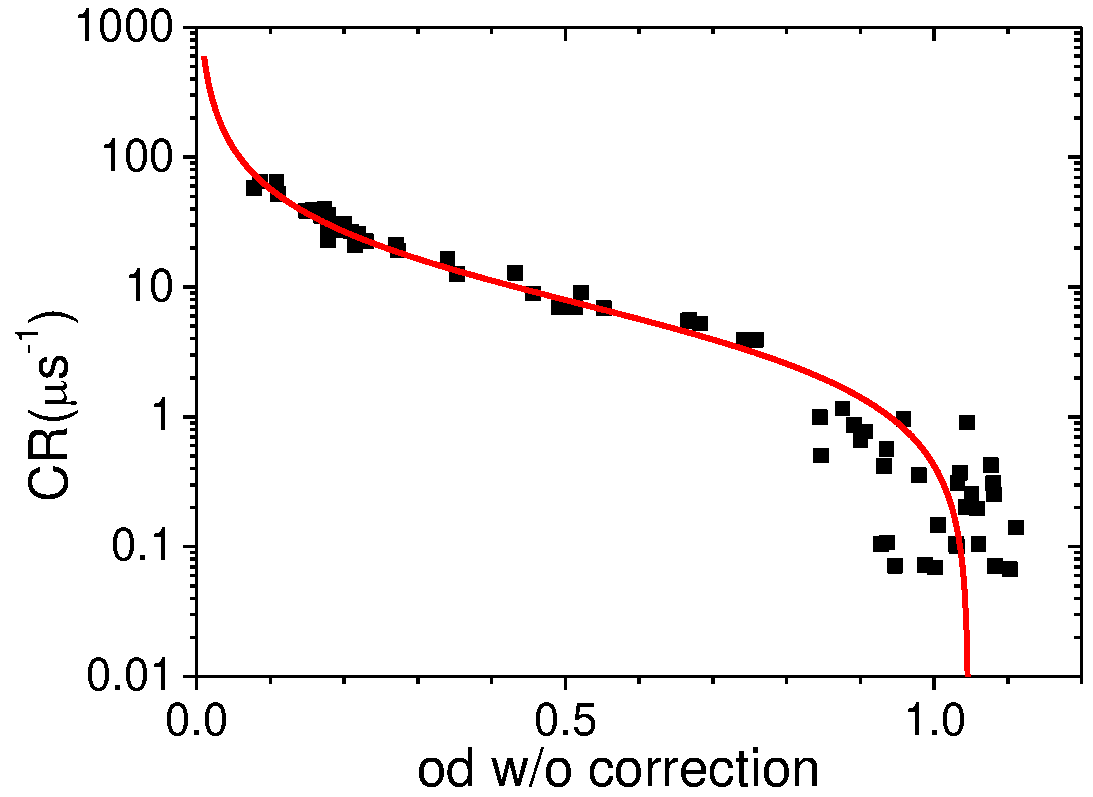
\includegraphics[width = 0.8\linewidth]{figures/Image_beta_calibration.pdf}
\end{center}
\caption{Image_beta_calibration}
\label{Image_beta_calibration}
\end{figure}


\section{CAMIMA: a multi-camera and image process platform}
\label{sec:camima}

% What is CAMIMA and why we need to develop it? (done 2021-8-27 18:27:20)
CAMIMA is a multi-camera control platform with image processing functions. Thanks to various camera adaptors provided by the Image Acquisition Toolbox, CAMIMA can support multiple camera types, including USB cameras from PointGrey, PCO and Migtex, Web camera and other general type of cameras. The primary time sequence is tailored for the absorption image for the cold atom experiment. After acquiring images from the camera, there are extendable and programable image processing functions for post-process images. Users can easily re-program the time sequence and processing sequence for various scenarios, e.g. denoising or de-fringe process, fluorescence image and so on.

% components description (done 2021-8-27 18:41:59)
The software is made of four parts: 
\begin{itemize}[noitemsep,topsep=0pt]
\item CAMIMA: Main control for converting data from different camera to a uniform image stream, which easier for following processing.
\item VUIMA: For showing and processing images from each image stream. VUIMA can be opened multiple.
\item CAMSET: Setting program for various cameras. Inside it, there is a general setting panel adaptation for specific type of camera.
\item FITSET: For general purpose fitting progress. fitting function can be edited as will.
\end{itemize}

\subsection{licensing, versions and updates}
% licensing (done 2021-8-27 18:42:40)
This programs is a free software: you can redistribute them and/or modify them under the terms of the GNU General Public License, version 3, as published by the Free Software Foundation. The full text of the license is available from \href{https://www.gnu.org/licenses/}{https://www.gnu.org/licenses/} and is included in the file COPYING included in the distribution.

% Version control (done 2021-8-27 18:42:47)
For adapting different version of MATLAB and its Appdesigner toolbox, this program is created with the following versions:
\begin{itemize}[noitemsep,topsep=0pt]
\item MATLAB2016
\item MATLAB2020
\end{itemize}

% download and updates (done 2021-8-27 18:42:51)
Software downloads and updates are made available via github:
\begin{itemize}[noitemsep,topsep=0pt]
\item \href{https://github.com/guozc12/CAMIMA}{https://github.com/guozc12/CAMIMA}
\end{itemize}

\subsection{Using the software: a basic guide}
\subsubsection{Prerequisites}
% prerequisite (done 2021-8-27 18:43:49)
Before installing CAMIMA, one need to install MATLAB with a version later than 2016. The listed several add-ons are needed.
\begin{itemize}[noitemsep,topsep=0pt]
    \item MATLAB (later than Ver. 2016)
    \item Appdesigner™ in MATLAB
    \item Image Acquisition Toolbox™ in MATLAB
    \item uitree in MATLAB
\end{itemize}

\subsubsection{Start CAMIMA}
% add Camima_main, i.e. main interface (done: 2021年8月4日21:43:37)
\begin{figure}[htb]
\begin{center}
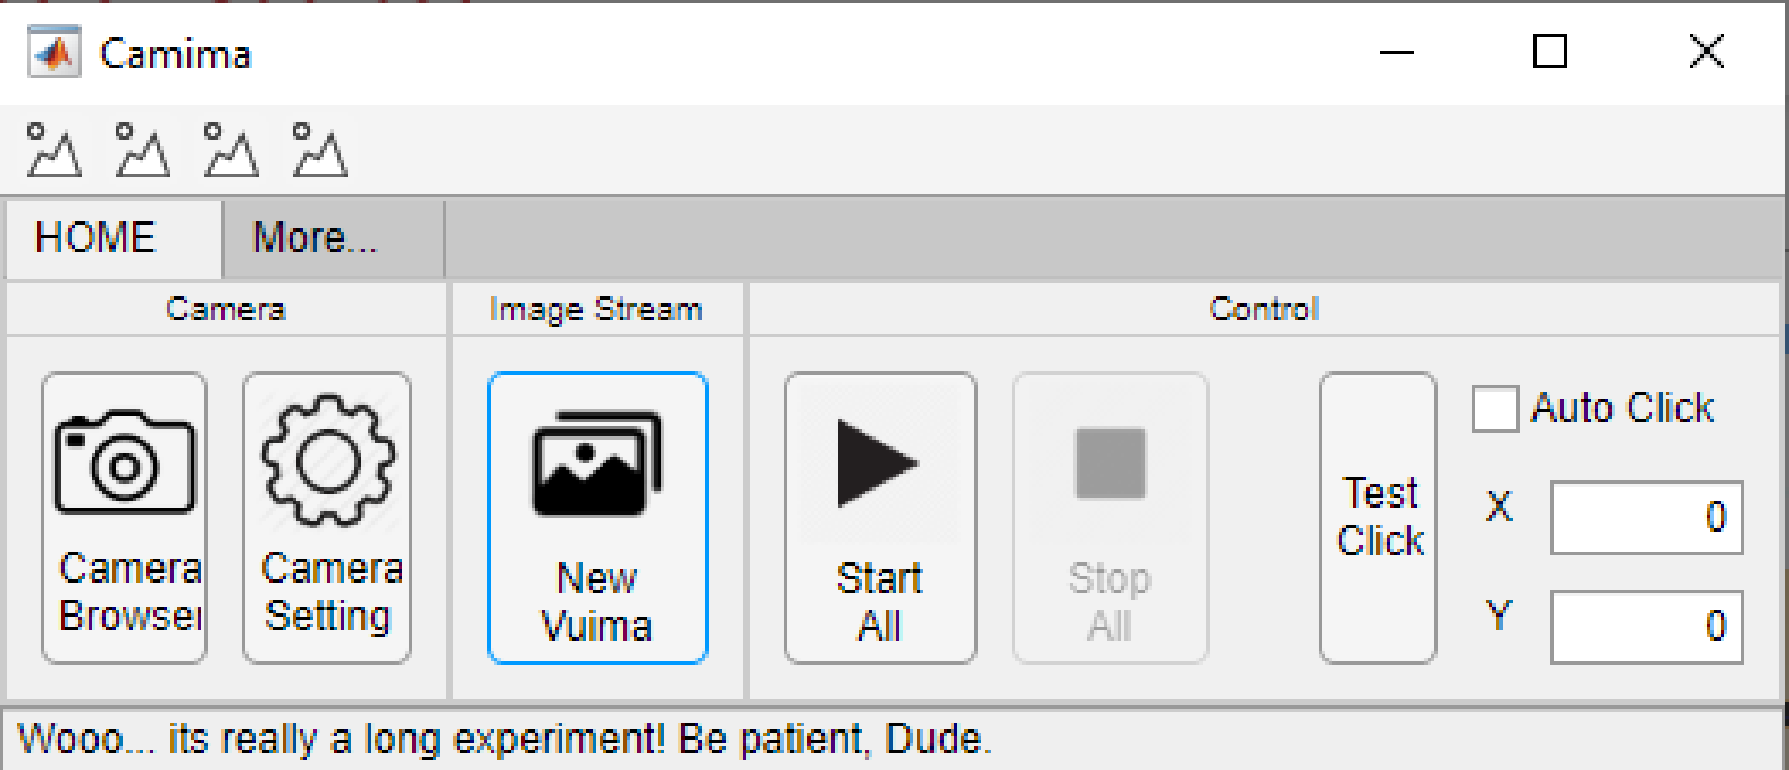
\includegraphics [width = 0.8 \linewidth]{Camima_main.pdf}
\end{center}
\caption[CAMIMA main panel]{CAMIMA Main panel.}
\label{Camima_main}
\end{figure}

% introducing the main panel (done: 2021年8月4日21:43:48)
Open the CAMIMA.mlapp in Appdesigner. Then click the Run button to run the main CAMIMA program. As shown in Fig. \ref{Camima_main}, a small panel shows you entrances for different functions:
\begin{itemize}[noitemsep,topsep=0pt]
    \item Camera Browser: Open a new panel for searching and initializing all installed cameras. (As shown in Fig. \ref{Camima_CamTree})
    \item Camera Setting: Open a new panel (CAMSET) to control each camera directly. (Fig. \ref{Camima_Camset})
    \item New VUIMA: Open an image processing panel (VUIMA) for viewing images and automatic image processing. (Fig. \ref{Camima_Vuima})
    \item Start All: For quick starting everything, including start acquisition for every camera
    \item Stop All: For quick stopping everything.
    \item Test Click: for setting a button, click after each shot with the written position on the right side.
\end{itemize}

% add Camima_CamTree, i.e. Camera browser (done 2021-8-29 11:57:06)
\begin{figure}[htb]
\begin{center}
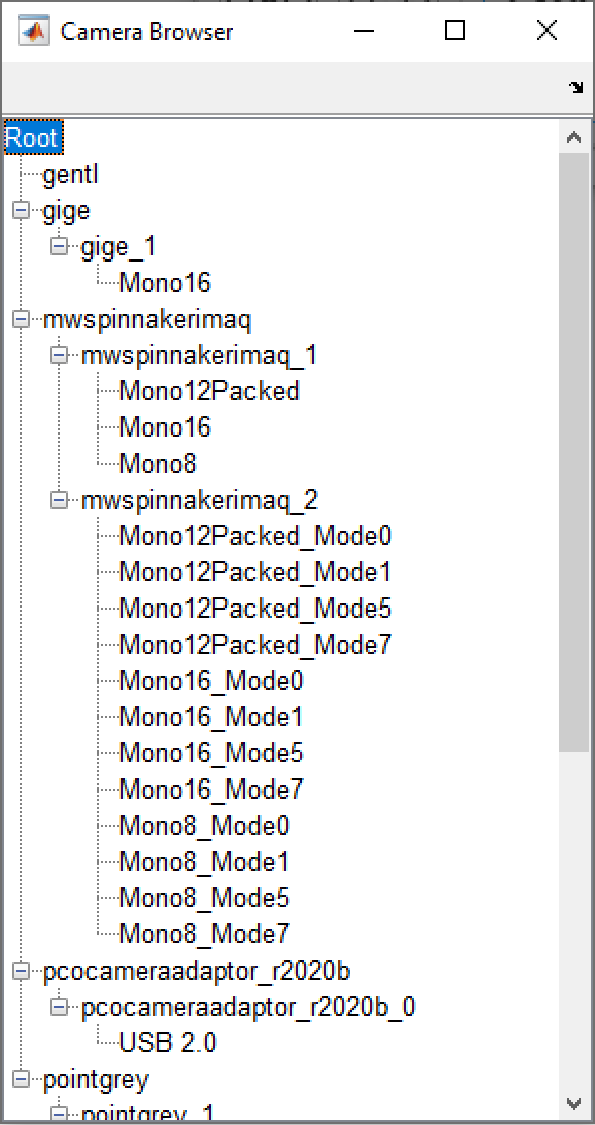
\includegraphics [width = 0.4 \linewidth]{figures/Camima_CamTree.pdf}
\end{center}
\caption[CamTree: show all available cameras for acquiring images]{CamTree shows all available cameras for acquiring images. When click the ``Camera Browser'' button in CAMIMA main panel, this tree window pops up and show you a full list of all available cameras.}
\label{Camima_CamTree}
\end{figure}

\subsubsection{Setting cameras by CAMSET}
% camera adaptors for different venders

\begin{itemize}[noitemsep,topsep=0pt]
    \item PointGrey
    \item BlackFly
    \item PCO camera
    \item Web Cam
    \item ...
\end{itemize}

% Control
As shown in Fig. \ref{Camima_Camset}, after catching each camera, we can control the camera manually, such as previewing, manual trigger for acquisition. For cameras from different vendors, the general settings are different. Thus, we generate a list in a new window, as shown in right panel of Fig. \ref{Camima_Camset}. User can change properties of camera, such as exposure time and binning. The ROI (Region-of-interest) can be set when camera is stop. More setting about automatic trigger can be set in the right-bottom panel of CAMSET window.

% add Camima_Camset, i.e. Camera setting (done 2021-8-29 11:50:03)
\begin{figure}[htb]
\begin{center}
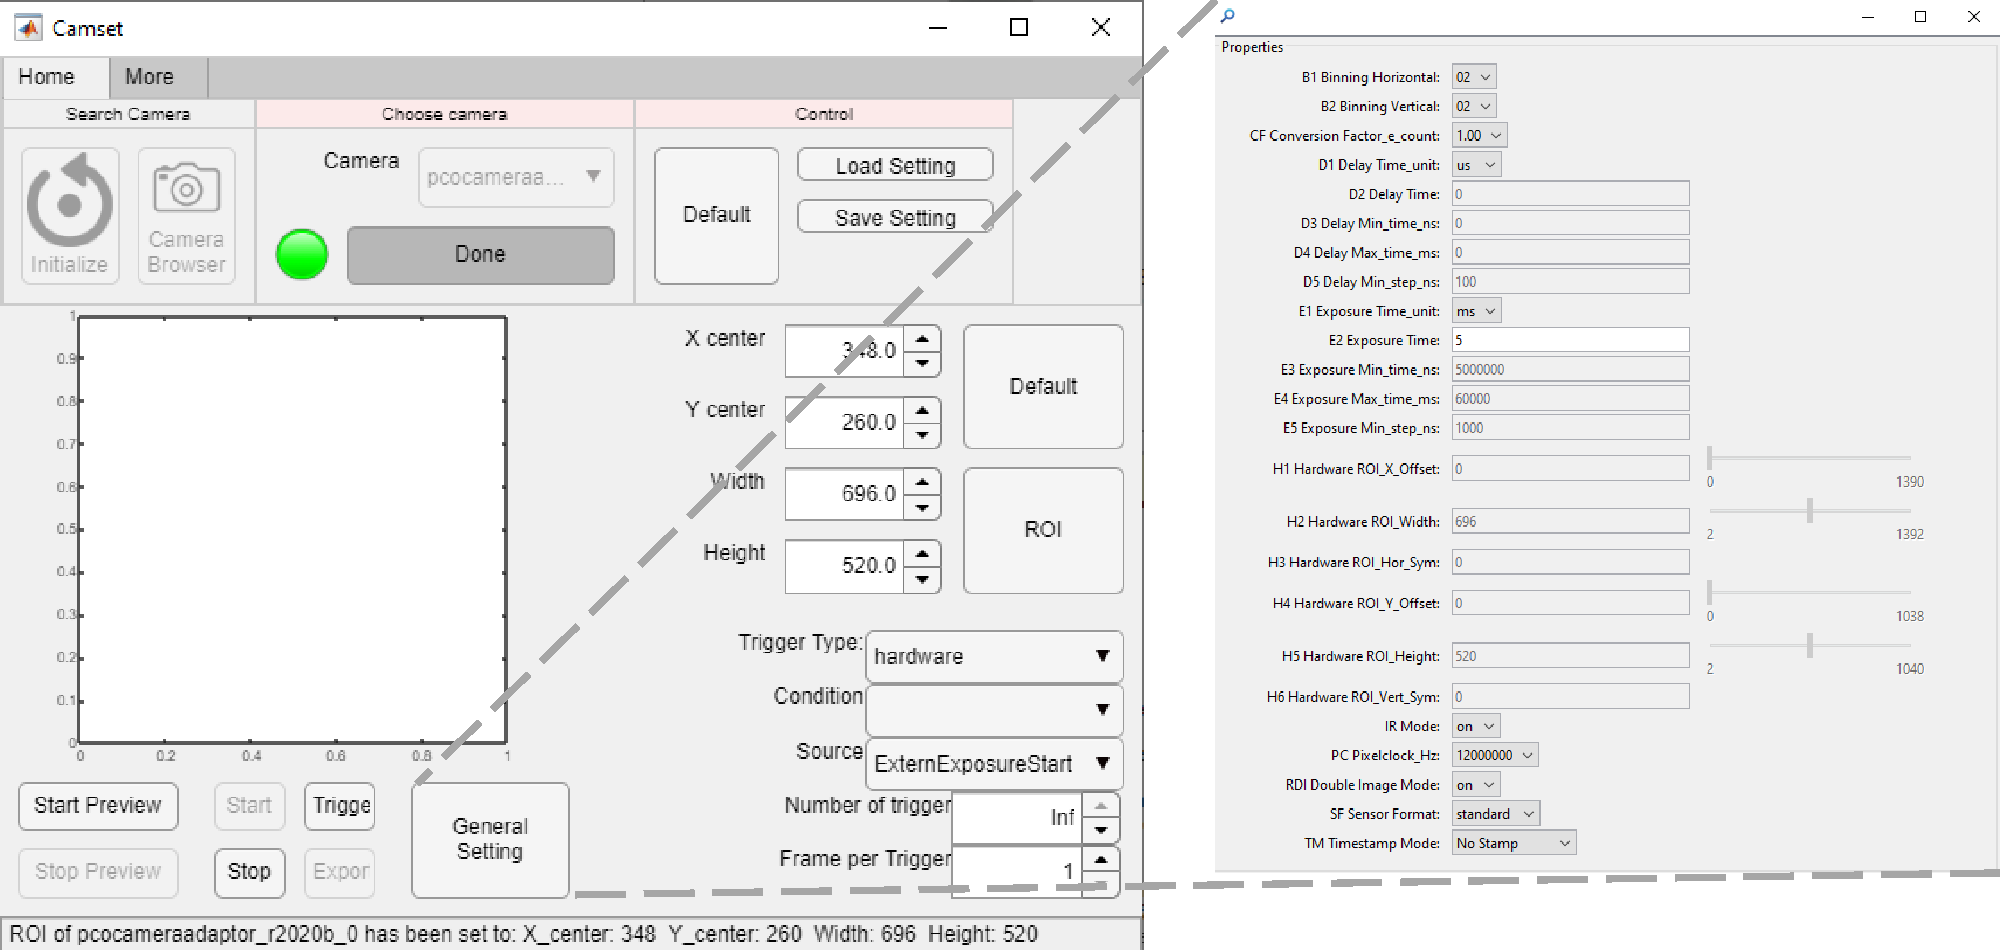
\includegraphics [width = \linewidth]{Camima_Camset.pdf}
\end{center}
\caption[CAMSET: a module of CAMIMA used to control and set cameras]{CAMSET is a module of CAMIMA used to control and set cameras. By switching the toggle, one can control multiple cameras. Besides the general setting, such as ROI and acquisition sequence, it also offers a specific entrance for each camera.}
\label{Camima_Camset}
\end{figure}

\subsubsection{Image acquisition}


% add Camima_Vuima, i.e. Viewing the image (done 2021-8-29 11:46:52)
\begin{figure}[htb]
\begin{center}
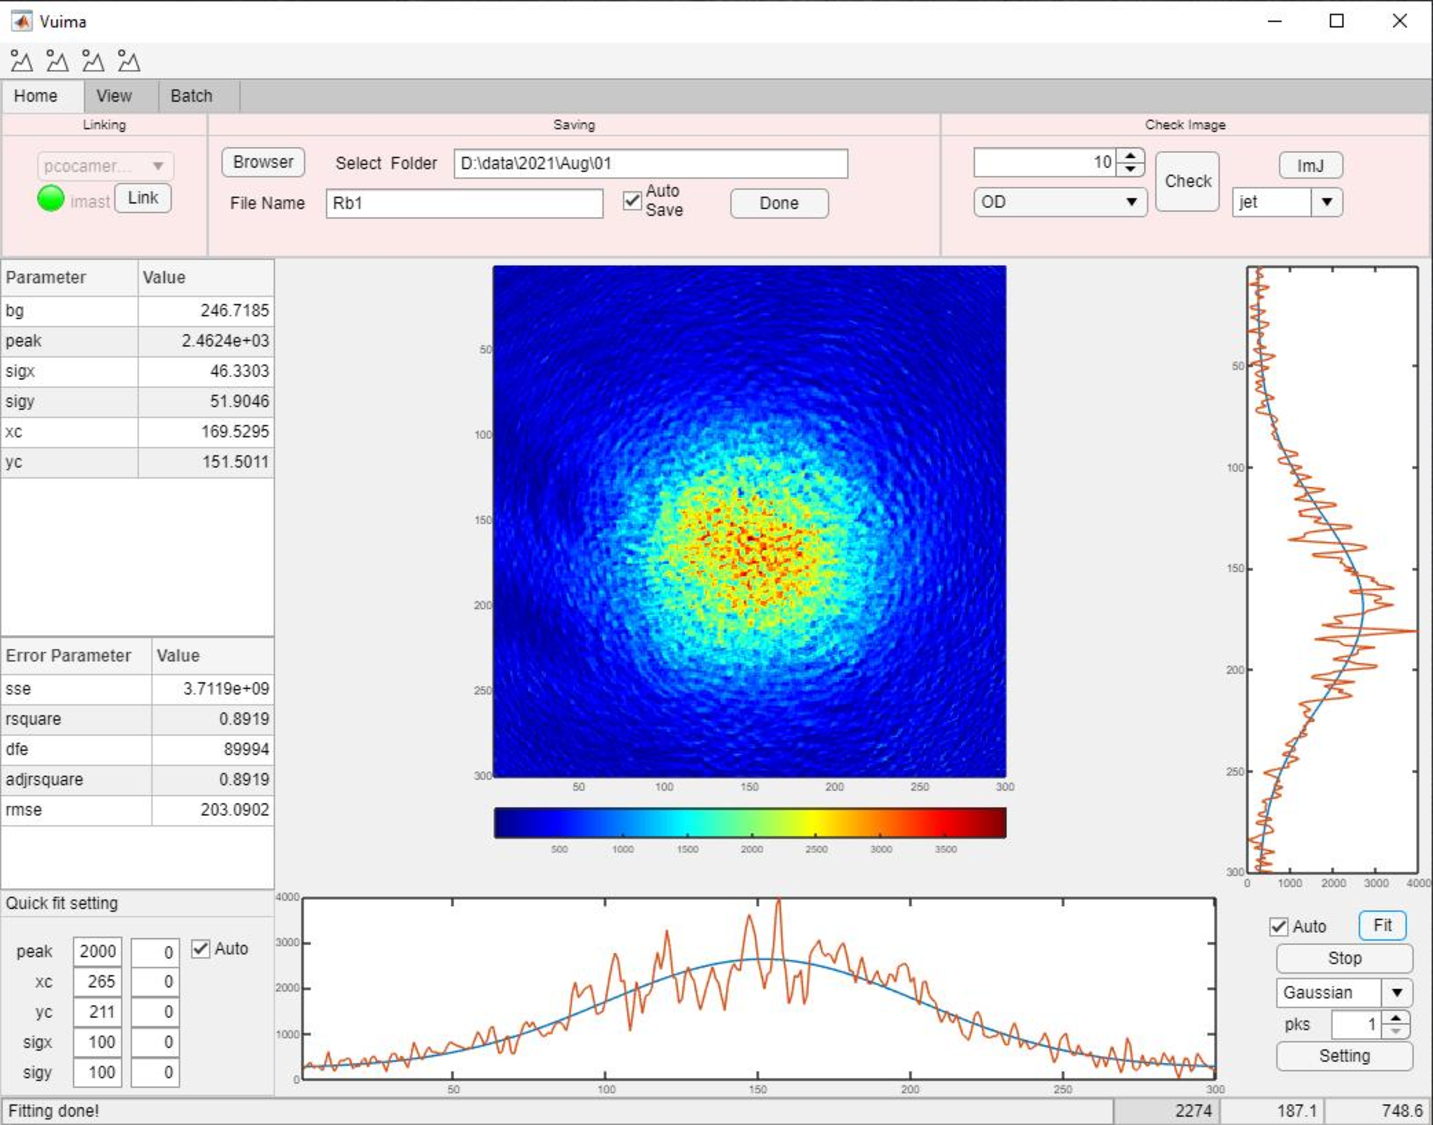
\includegraphics [width = \linewidth]{Camima_Vuima.pdf}
\end{center}
\caption[VUIMA: a module of CAMIMA used to preview image]{VUIMA is a module of CAMIMA used to preview image. The VUIMA window can be opened multiple for each image stream. Besides previewing the image, it can show the fitting results comparing to the raw data. It offers entrance for setting arbitrary fitting function.}
\label{Camima_Vuima}
\end{figure}

1. time sequence of image acquisition
2. converting camera data to image stream
3. show and pre-process of images on VUIMA

\subsubsection{post processing of image}

% add Camima_Fitset, i.e. Setting the fitting (done 2021-8-29 11:54:52)
\begin{figure}[htb]
\begin{center}
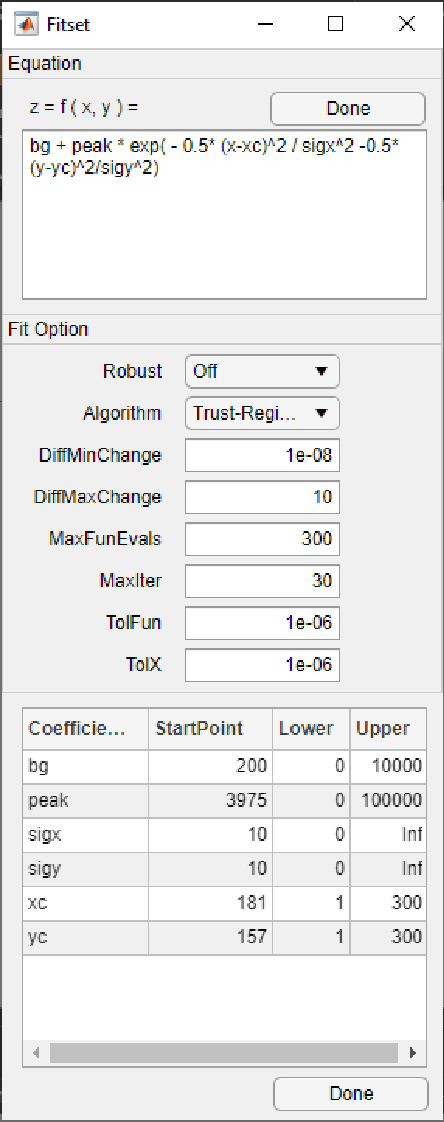
\includegraphics [width = 0.4\linewidth]{Camima_Fitset.pdf}
\end{center}
\caption[FITSET: a module of CAMIMA used to set arbitrary fitting function]{FITSET is a module of CAMIMA used to set arbitrary fitting function. Besides the default fitting functions written under the toggle button, this module offers function for easily generate arbitrary fitting function.}
\label{Camima_Fitset}
\end{figure}

1. statistic data from image
2. fitting of image
3. batch processing

\section{Fast magnetic field control}
\label{sec:fastcoil}

% why we need fast-magnetic control
As we mentioned in the section about Feshbach resoannce, by tuning magnetic field we can easily control the scattering properties of atoms, i.e. the interacrion strength. In the precious set-up, we use a large Helmhotz coil with about 90(check) turns. The inductance of the coil is typically 2 mH(need check), which is a very large one with long time contants. (find a better way to describe here). So, even with driver with 100V(check), we will have a rising slope with 1ms(..), which is not fast enough for our requirement to control the interaction. Our request is depend on the time scale of the research object. For example, a typical BEC with as of 100 a0 order will have time scale less than 1 ms. Thus, to control the interaction fast we need about time scale 10 us or even faster. Then we can make sure the sample's size of other paraters changing much slower than the interaction changing.

\subsection{Fast-B coil design and driver}

% What is fast coil and how to build one.
So, with the above request, we need to build another coil which can generate a small but fast magnetic field. The limitation is inductance of the coil, so we reduce its winding to as few as possible. However, with fewer tunes the magnetic field it can generate all declines. So we need make a trade off here. As plotted in the following graph. we can find that their is a best tunes to generate the B-field we want. (Add Figures here) Also, to generate larger magentic field, we put it as close as posible to the cell. Finally, we choose a Helmhots coil with 6 turns in each set. The set-up with Main Feshbach coil is shown here. To adapt our previous large coil. we design a holder made of 聚酰乙烯,查一下是什么。and the holder winding with fast coil is steaked into the 2 inch optical path for MOT beam. 

% current driver and its test data
To driver this fast coil, we need a current driver which can generate fast change of current, so with Lintao's help, we design a fast coil driver with several group of JFET for fast turning on-off and also make a precision control of the current with very few leaking current. The driver schematic can be found in the appendix.C(add here)

% coupling of fast coil and main coil
As shown in JILA's thesis, now, we need to consider the coupling of the fast coil and the main coil and the environment. Since, these coupling will cause oscillation and jiggle when quenching the current in the fast coil. As modeled by the 集总 elements, as shown in figure. (Add figure). The coupling from the main coil and fast coil can be viewed as ... and environment as ... Finally, we have a tested quenching for fast coil.



\subsection{Dynamic compensation for induced and eddy current}
% Why we need dynamic compensation
There are two reasons for us to do the dynamic compensations, first is the coupling of fast coil and main coil and the environment will cause a jigger when we quench the current of the fast coil. To avoid this jigger, we 

\section{Other Technical Issues}
\subsection{Magnetic field gradient compensation}
\label{subsec:gradientcompen}
%Why we need to compensate the B-field gradient 
As mentioned before, we use a pair of Feshbahc coil to generate large bias magntic field to control the Feshbach resonance. However, due to the imperfection of the coil, such as assymetry of each up and down coils and distance not coincident with the Helmhotz coil, the magnetic field typically has a gradient and/or curvature onto the atom. This effect can be easily detect by free-falling of atom in high magnetic field. If one find that the accelaration of the atom is deviated from gravity accelaration, there must be the gradient. Another evidence is the MW (rf) spectroscopy for a elongated sample which could detect the gradient on the horizontal direction. As shown in Figure, we free-fall Rb or Na under high magnetic field, and the accelaration is shown to be differnt from gracity, thus, in our set-up this effect could affect a lot when doing the following experiment with free-falling method. (give more number) 

% What is our gradient looks like?
Before talking about canceling this gradient, we first try to measure it. The method is simple following the MW transition calibration method. We apply the MW pulse coupled the 1,-1 and 2,0 state. Then to get the spacial distribution of the magentic field, we first let the atom free-falling, then apply the MW pulse at differnt ToF. Even though the gradient will affect the position of the atom, considering the samll effect related to g, this can be neglected. Then, we get the magnetid spactial distribution as show in Figure. We can see that there is not only a gradient of the magnetic field but also does the curvature. By a simple quadratic cruve fitting we get the curvature about 1xxx \(G/cm^2\) and an average gradient about xx G/cm. One thing need to be notice here is what we measrued is only the magnetic field gradient on vertical direction, which is the mainly contribution in our case. As we can see in the horizontal direction the accelaration is even much lower than that in veritical direction which infer that this gradient should comes mainly from the wrong distance of the Helmhotz coil.

% How to compensate the grdient and cuvarture
As it is hard to compensate the full of the curvature since to compensate the curvature we need fully recover the helmhotz condition which need much larger magnetic field compare to the several hundred gauss magnetic field. So, to 妥协性质地 solve the question we meet, we degenerate to compensate the avarage gradient to zero inside the interesting ToF we care. So, we can just add a another magnetic gradient on the vertical direction and to change the value of this gradient to find the best compensate point. For the first test, we simply use the half of our up and down shim coil (e.g. up coil). As shown in Figure, we can generate a inversely direction gradient oppposite to the main coil. Then, we simply change the current of the shim coil and test the accelarion of the atom, to find the compensation point. As the dipole moment of Na and Rb is quite different, we can also find the intersect point of them which represents zero average gradient compensation point, as shown in Figure. Finally, we tune the shim coil to the current at the in tersrct and remeasrue the magnetic field with MW spectroscopy method and compare the result with previous non-compensation one as shown in Figure. It is obvious the mean graditn is reduced a lot however the curvature is still there. The compensated gradient and curture is about xxx \(G/cm^2\) and \(xxx G/cm\) now which should be enough for observing BEC mixture free-falling. 

\subsection{Microwave full-wave loop antenna}
\label{subsec:FWLA}
% Why we need to build the 2.57GHz and 7.5GHz full-wave loop antenna
As described in Section.xx, the internal states of atom can be controlled by electromagnetic wave. Typically to drive transition between two different hyperfine states, we need use micro-wave(MW) which typical has wavelength about 0.3 m to 3 m, i.e. 300MHz to 300 GHz for frequency in vacuum. For Na and Rb atom, the hyperfine splittings are 1.7 GHz and 6.8 GHz at zero magnetic field. When magnetic field increasing to 350 G (since we typically use the 347 G Feshbach resonance to control the inter-species interaction), the splitting between F=1, mF=1 and F=2, mF=2 states are 2.6 GHz and 7.5 GHz for Na and Rb separately. Thus, we need an antenna which can work well at these frequency. Here, "work well" commonly has two meanings: one is the antenna's standing wave ratio (SWR) is approaching 1, which means it can transmit more power to emitting as EM wave instead of reflecting them back to the power amplifier. Secondly, we need the atom feel the largest amplitude of E-field because the transitions between different F-state is mainly connected be electron dipole, i.e. an electrical dipole transition.(here, need more carefully check) So, the antenna's position, including its distance to atom and its direction angle are both critical to maximum the utility of the antenna. We can define the efficiency fot the above two process as $\mu_trans$ and $\mu_anta$, and the total efficiency is just the multiplication of them.

% talk about near-field and far-field difference
A commercial antenna is typically designed to work well at far field. The radiation power declines inversely proportional to the distance. Thus, in order to increase the power received by atom, we need to put the antenna as close to the atom as possible. However, this renders the radiation felt be the atom turns to be near-field instead of far-field. As depicted in Figure, the electric and magnetic field line (OK?) of a dipole antenna is plotted as blue and red separately. At a large distance of the antenna, the electric field line is almost perpendicular to the \(\hat{r}\) direction. However, when getting closed, it shows more portions to the \(\theta\) direction. This tells us that near-field electromagnetic field of antenna behaves quite different from its far-field one. At far-field region, both electric and magnetic field lines are perpendicular to the Poynting vector, which shows its radiation properties. However, the near-field cannot be treated as a radiation, instead, we typically treat it as "quasi-static" field. A quasi-static field means the distribution of EM field is the same as it in electrostatics, except a oscillation in magnitude with \(e^{i\omega t}\). In engineering, these study is important to wireless-charging, proximity sensors and so on.

% what previous one done, and what's the problem of it
Previously, we use horn antenna for Rb MW transition at 6.8GHz. (add reference here) The distance between horn and atom is about 10-15 cm (check and measure the number). Problem to put the antenna closer to the atom is its huge size which could block the optic path and its metallic body could disturb the strong magnetic field of large Feshbach coil causing a gradient on atom. So the nearest position we can put is about (10 cm) and the measurement Rabi frequency of Rb 1,1 to 2,2 transition at 350 G (7500 GHz) is less than 10kHz (check the number) with a 40 W power amplifier. The correspondents half-\(\pi\) pulse duration is about 50us (check number) which is too long for most of our experiment such as high magentic field image or too weak for dissociating the FR molecule. Thus, we need upgrade it to enhance the Rabi frequency.

% How to improve? what is full-wave loop antenna?
So, a naive solution is try to put the antenna as close to the cell as possible and try to shrink its size smaller and thinner. Therefore, the loop antenna will be a proper choice. A loop antenna is just a simple loop connected to the signal generator. However, for our case with frequency at 2.6 GHz and 7.5 GHz, The wavelength is around several cm to tens of cm. This is comparable to our coil size, which could introduce severe problem on impedance matching. A common solution is making the perimeter of the loop antenna just a full wavelength, which called the full-wave loop antenna. As shown in Figure (add figure), xxxx. when the scale of antenna is closed to wavelength, the distribution of radiation becomes quite different to those samll-loop antenna. This can be explained by a simplified picture, as shown in Figure. at the 接头地方和正对面 current changes with largest amplitude, and there placed two nodes at the quarter wavelength place to the 接头处。However, for small-lopp antenna, the current almost have same phase on the whole coil. Therefore, they have different patterns shown in Figure.

% How the antenna works?
According to the near-field quasi-static EM field theory, we can write down the EM field as following:
\begin{equation}
    E...
\end{equation}
Then, we can plot the radiation power as function of distance to the center of the loop coil, as shown in Figure. The maximum radiation appears at \(\lambda/4\) away from the plane of coil. And actually, the power at the center of coil is zero, which is in opposite to the case of a small-loop coil. For our case with f=2.6GHz, the wavelength is about 12 cm and we place the coil 3 cm away from atom to achieve the largest power. For the 7.5Ghz case, we use paramter about 4 cm coil loop, however we cannot put the coil 1 cm away from the atom since the cell has a size of 2cm, so 综合考虑optical path and power, we put the tiny coil at the side of cell with a 45 degree angle and distance to atom about 3 cm. 

% Set-up and impedance matching
After preparing the coil, we set up the standard MW power amplifier circuit for it. For the 2.6Ghz one, we use (link) from Taobao, and for the 7.5 Ghz one, we use .. from ... Before the amplifier we add a switch controlled by TTL signal and finally the signal generator is SG386. The key point to increase the efficiency from power amplifier to the coil, i.e. \(\eta_{trans}\), we need carefully consider the impedance matching from the transmission wire to eh loop coil. As shown in Figure, we demonstrate several full-wave loop antenna with different shapes. They have different impedance, the ideal one is the rectangular with aspect ratio 1:2, which just have 50 Ohm impedance. However, for our case with round shape, we have the coil with 133 Ohm. our transmission line and power amplifier are all 50 Ohm, so we need to do the impedance matching. Typical we can use a baloon, to simplify we use a 75 Ohm transition line to enhance the transmission rate. As shown in Figure, the signal can be reflected at the boundary of two lines with different impedance, and from 50 ohm to 75 Ohm wire and from 75 ohm to the 133 ohm coil, there exist two reflection wave. If we choose the length of the 75 Ohm line, we can cancel the reflection by superposition two of them. 

% How detail the impedence mathcing works
要配上公式和图片解释这个事情

% Test of the coil
Even though now we know how long the q-section line should be, we still need to do the off-line test for its performance, because a several cm length is to short to allow several uncertainty such as length uncertaainty and 衔接 place different impendence. These imcomplete can cause the phase of replectiong wave shifting and decline the effect of impedence matching. Therefor, we build a series of coil with different length of its q-section, and measrure its return loss rate by a directional coupler. As shown in Figure, we send the siganl into the outpur port of a coupler and the refleting wave from the antenna (connecting on the input port of coupler) will coupled a small portion in to the coupled port and detected by an analyser spectrum. By calculating the reflecting power and injection power, we plot the return loss rate as a function of the length og the q-section line. We can see the period does refer to the half of wavelength and there is a shift which could be attribute the imperfection of q-section line. By fitting with a sine function, we extract the 周期,shift 等等,在列表里。 So, We can now build the coil with lowest return loss for covering our usage frequency.

% Online test
Finally, we put the coil onto the atom cell. First, we test the transmission rate of the coil online to make suere the impedance matching works well, since the offline test with an enviroment open, however the online environment is full of different metals around the coil which could change the boundary condition and shift the impedance of the coil. So, we use the same mathod to test the transmision rate of the coil as shown in Figure. The bandwidth is about xxx MHz. Then, we test the Atomic Rabi frequency to measure the final performance of the coil. We apply the MW pulse for Na at 350 G and get the rabi frequency at different freq or detuning?. As shown in Figure, we test the saturation power and get a Rabi maximum to about 100kHz(check the number). This could allow us to make a pi pulse within 10 us which is enough for most case such as optical pumping in high field and also for MW spectroscopy??.

% about 6.8 7.5Ghz coil
By comfirming the 2.6 GHz coil can work, we turn to use build the 7.5 GHz coil, which could increase the Rabi freq for Rb at high field too. So, we build a similar coil with parameter about 4 cm and its q-section about xx cm, this coil is rather too samll even to put it onto the cell, because it will definitely block some part of the MOT beam. So, finally, we decide to sacrifies some power to put the coil a little bit further away from the coil, i,e, at the corner of the cell, whcih increase the distance of the coild to about 3 cm. Best working distance for the 7.5 Ghz coild should be \(\lambda/4\), i.e. 1 cm, so for 3cm distance we get a power about 1/3 compare to the maximum one (need check number). 总的来说,最后test of the rabi freq is about 100kHz, which recover the previous horn antenna performance. which could allow us to remove the horn antenna (even the coil is working on resonace at 7.5 GHz, when 6.8 Ghz it still can work with a transition rate about \(xxx\%\), so for a typical MW evaporation whichi only consumpted very small power 是足够用的了)

% https://www.everythingrf.com/community/what-is-the-difference-between-a-monopole-and-dipole-antenna
\begin{figure}[htb]
\begin{center}
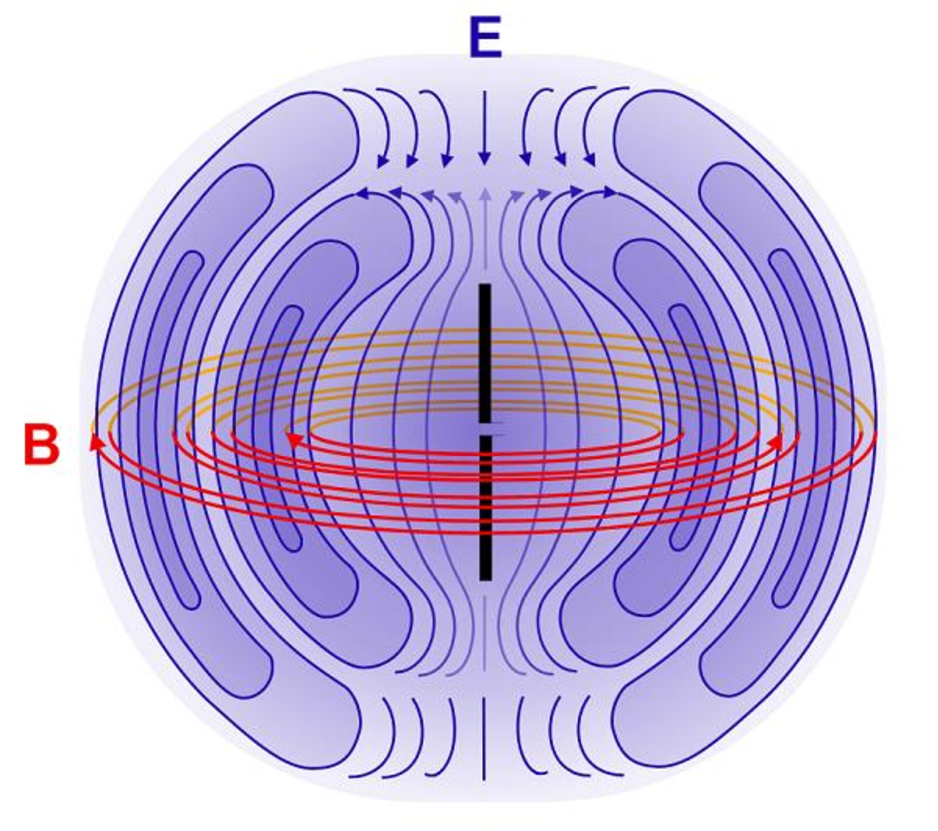
\includegraphics [width =0.5 \linewidth]{Apparatus-EM_field_antenna.pdf}
\end{center}
\caption{}  
\label{antenna_EM}
\end{figure}


\begin{figure}[htb]
\begin{center}
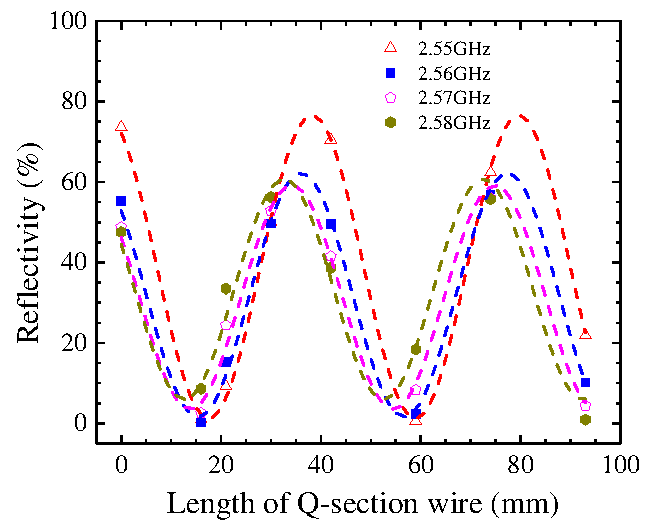
\includegraphics [width =0.7 \linewidth]{Apparatus-loop_antenna_retrun_loss.pdf}
\end{center}
\caption{}  
\label{antenna_return_loss}
\end{figure}

\begin{figure}[htb]
\begin{center}
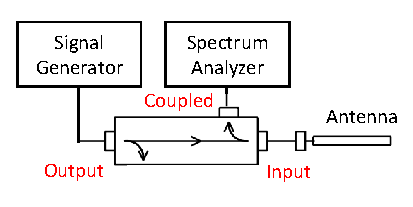
\includegraphics [width =0.7 \linewidth]{Apparatus-measure_SWR.pdf}
\end{center}
\caption{}
\label{SWR_measure_method}
\end{figure}


% How to build the 
